
%% Projectile Questions used on the
%% NYSED Physics Regents Examination
%%--------------------------------------------------

%% this section contains 54 problems


%% Section June2015
%%--------------------
\element{nysed}{
\begin{question}{June2015-Q38}
    Without air resistance, a kicked ball would reach a maximum height of \SI{6.7}{\meter} and land \SI{38}{\meter} away.
    With air resistance, the ball would travel:
    \begin{choices}
        \wrongchoice{\SI{6.7}{\meter} vertically and more than \SI{38}{\meter} horizontally.}
        \wrongchoice{\SI{38}{\meter} horizontally and less than \SI{6.7}{\meter} vertically.}
        \wrongchoice{more than \SI{6.7}{\meter} vertically and less than \SI{38}{\meter} horizontally.}
      \correctchoice{less than \SI{38}{\meter} horizontally and less than \SI{6.7}{\meter} vertically.}
    \end{choices}
\end{question}
}


%% Section June2014
%%--------------------
\element{nysed}{
\begin{question}{June2014-Q47}
    Which combination of initial horizontal velocity, ($v_h$),
        and initial vertical velocity, ($v_v$), results in the greatest horizontal range for a projectile over level ground?
    [Neglect friction.]
    \begin{multicols}{2}
    \begin{choices}
        \AMCboxDimensions{down=-1.5em}
        \correctchoice{
            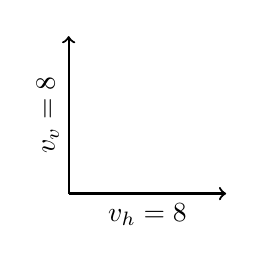
\begin{tikzpicture}
                \draw[white] (-0.5,-0.5) rectangle (2.1,2.1);
                \draw[thick,->] (0,0) -- (90:2cm);
                \node[anchor=south,rotate=90] at (90:1cm) {$v_v=\SI{8}{\meter\per\second}$};
                \draw[thick,->] (0,0) -- (0:2cm);
                \node[anchor=north] at (0:1cm) {$v_h=\SI{8}{\meter\per\second}$};
            \end{tikzpicture}
        }
        \wrongchoice{
            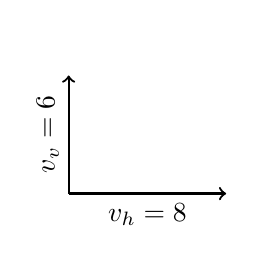
\begin{tikzpicture}
                \draw[white] (-0.5,-0.5) rectangle (2.1,2.1);
                \draw[thick,->] (0,0) -- (90:1.5cm);
                \node[anchor=south,rotate=90] at (90:0.75cm) {$v_v=\SI{6}{\meter\per\second}$};
                \draw[thick,->] (0,0) -- (0:2cm);
                \node[anchor=north] at (0:1cm) {$v_h=\SI{8}{\meter\per\second}$};
            \end{tikzpicture}
        }
        \wrongchoice{
            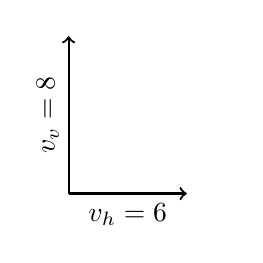
\begin{tikzpicture}
                \draw[white] (-0.5,-0.5) rectangle (2.1,2.1);
                \draw[thick,->] (0,0) -- (90:2cm);
                \node[anchor=south,rotate=90] at (90:1cm) {$v_v=\SI{8}{\meter\per\second}$};
                \draw[thick,->] (0,0) -- (0:1.5cm);
                \node[anchor=north] at (0:0.75cm) {$v_h=\SI{6}{\meter\per\second}$};
            \end{tikzpicture}
        }
        \wrongchoice{
            \begin{tikzpicture}
                \draw[white] (-0.5,-0.5) rectangle (2.1,2.1);
                \draw[thick,->] (0,0) -- (90:1.5cm);
                \node[anchor=south,rotate=90] at (90:0.75cm) {$v_v=\SI{6}{\meter\per\second}$};
                \draw[thick,->] (0,0) -- (0:1.5cm);
                \node[anchor=north] at (0:0.75cm) {$v_h=\SI{6}{\meter\per\second}$};
            \end{tikzpicture}
        }
    \end{choices}
    \end{multicols}
\end{question}
}


%% Section June2013
%%--------------------
\element{nysed}{
\begin{question}{June2013-Q05}
    A projectile is launched at an angle above the ground.
    The horizontal component of the projectile's velocity, $v_x$, is initially \SI{40}{\meter\per\second}.
    The vertical component of the projectile's velocity, $v_y$, is initially \SI{30}{\meter\per\second}.
    What are the components of the projectile's velocity after \SI{2.0}{\second} of flight?
    [Neglect friction.]
    \begin{choices}
      \correctchoice{$v_x=\SI{40}{\meter\per\second}$ and $v_y=\SI{10}{\meter\per\second}$}
        \wrongchoice{$v_x=\SI{40}{\meter\per\second}$ and $v_y=\SI{30}{\meter\per\second}$}
        \wrongchoice{$v_x=\SI{20}{\meter\per\second}$ and $v_y=\SI{10}{\meter\per\second}$}
        \wrongchoice{$v_x=\SI{20}{\meter\per\second}$ and $v_y=\SI{30}{\meter\per\second}$}
    \end{choices}
\end{question}
}

\element{nysed}{
\begin{question}{June2013-Q06}
    A ball is thrown with an initial speed of \SI{10}{\meter\per\second}.
    At what angle above the horizontal should the ball be thrown to reach the greatest height?
    \begin{multicols}{4}
    \begin{choices}
        \wrongchoice{\ang{0}}
        \wrongchoice{\ang{30}}
        \wrongchoice{\ang{45}}
      \correctchoice{\ang{90}}
    \end{choices}
    \end{multicols}
\end{question}
}


%% Section June2012
%%--------------------
\element{nysed}{
\begin{question}{June2012-Q45}
    The diagram below represents a setup for demonstrating motion.
    \begin{center}
        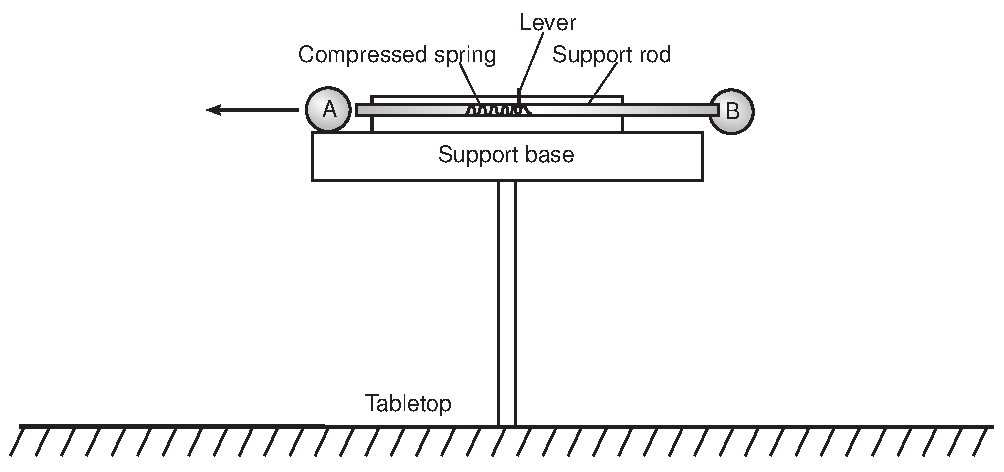
\includegraphics[keepaspectratio,width=0.95\linewidth]{June2012-Q45}
    \end{center}
    When the lever is released, the support rod withdraws from ball $A$, allowing it to fall.
    At the same instant, the rod contacts ball $A$, propelling it horizontally to the left.
    Which statement describes the motion that is observed after the lever is released and the balls fall?
    [Neglect friction.]
    \begin{choices}
        \wrongchoice{Ball $A$ travels at constant velocity.}
      \correctchoice{Ball $A$ hits the tabletop at the same times as ball $B$.}
        \wrongchoice{Ball $B$ hits the tabletop before ball $A$.}
        \wrongchoice{Ball $B$ travels with an increasing acceleration.}
    \end{choices}
\end{question}
}


%% Section June2011
%%--------------------
\element{nysed}{
\begin{question}{June2011-Q11}
    Four identical projectiles are launched with the same initial speed, $v$,
        but at various angles above the level ground.
    Which diagram represents the initial velocity of the projectile that will have the largest total horizontal displacement?
    [Neglect air resistance.]
    \begin{multicols}{2}
    \begin{choices}
        \AMCboxDimensions{down=-1.5em}
        \wrongchoice{
            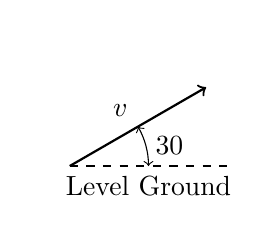
\begin{tikzpicture}
                \draw[white] (-1.5em,-1.5em) rectangle (2,1.75);
                \draw[dashed] (0,0) -- (2,0) node[pos=0.5,anchor=north] {Level Ground};
                \draw[thick,->] (0,0) -- (30:2) node[pos=0.5,anchor=south east] {$v$};
                \draw[<->] (1,0) arc (0:30:1) node[pos=0.5,anchor=west] {\ang{30}};
            \end{tikzpicture}
        }
        \correctchoice{
            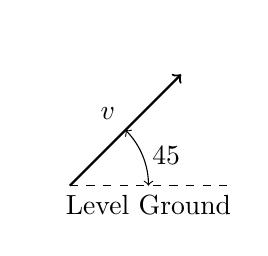
\begin{tikzpicture}
                \draw[white] (-1.5em,-1.5em) rectangle (2,2);
                \draw[dashed] (0,0) -- (2,0) node[pos=0.5,anchor=north] {Level Ground};
                \draw[thick,->] (0,0) -- (45:2) node[pos=0.5,anchor=south east] {$v$};
                \draw[<->] (1,0) arc (0:45:1) node[pos=0.5,anchor=west] {\ang{45}};
            \end{tikzpicture}
        }
        \wrongchoice{
            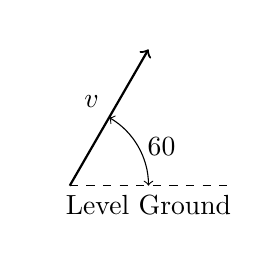
\begin{tikzpicture}
                \draw[white] (-1.5em,-1.5em) rectangle (2,2);
                \draw[dashed] (0,0) -- (2,0) node[pos=0.5,anchor=north] {Level Ground};
                \draw[thick,->] (0,0) -- (60:2) node[pos=0.5,anchor=south east] {$v$};
                \draw[<->] (1,0) arc (0:60:1) node[pos=0.5,anchor=west] {\ang{60}};
            \end{tikzpicture}
        }
        \wrongchoice{
            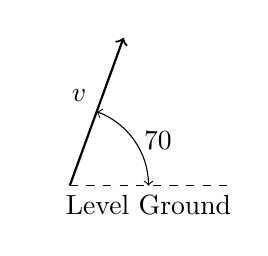
\begin{tikzpicture}
                \draw[white] (-1.5em,-1.5em) rectangle (2,2);
                \draw[dashed] (0,0) -- (2,0) node[pos=0.5,anchor=north] {Level Ground};
                \draw[thick,->] (0,0) -- (70:2) node[pos=0.5,anchor=south east] {$v$};
                \draw[<->] (1,0) arc (0:70:1) node[pos=0.5,anchor=west] {\ang{70}};
            \end{tikzpicture}
        }
    \end{choices}
    \end{multicols}
\end{question}
}


%% Section June2010
%%--------------------
\element{nysed}{
\begin{question}{June2010-Q06}
    As shown in the diagram below,
        a student standing on the roof of a \SI{50.0}{\meter} high building kicks a stone at a horizontal speed of \SI{4.00}{\meter\per\second}.
    \begin{center}
    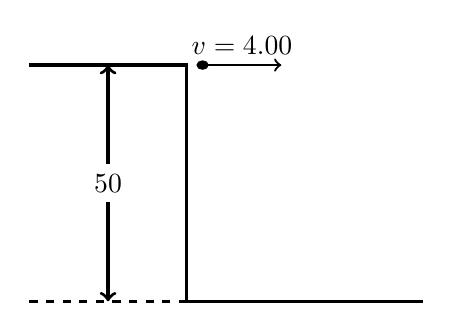
\begin{tikzpicture}[yscale=0.75]
        \draw[very thick] (-2,0) -- (0,0) -- (0,-4) -- (3,-4);
        \draw[fill] (0.2,0.0) circle [radius=2pt];
        \draw[thick,->] (0.2,0.0) -- ++ (0:1)
            node[anchor=south] at ++ (0:-0.5) {$v=\SI{4.00}{\meter\per\second}$};
        \draw[very thick,dashed] (-2,-4) -- (0,-4);
        \node (A) at (-1,-2.0) {\SI{50}{\meter}};
        \draw[very thick,->] (A) -- (-1,0);
        \draw[very thick,->] (A) -- (-1,-4);
    \end{tikzpicture}
    \end{center}
    How much time is required for the stone to reach the level ground below?
    [Neglect friction.]
    \begin{multicols}{2}
    \begin{choices}
      \correctchoice{\SI{3.19}{\second}}
        \wrongchoice{\SI{5.10}{\second}}
        \wrongchoice{\SI{10.2}{\second}}
        \wrongchoice{\SI{12.5}{\second}}
    \end{choices}
    \end{multicols}
\end{question}
}

\element{nysed}{
\begin{question}{June2010-Q14}
    Four projectiles, $I$, $J$, $K$, and $L$,
        were launched from, and returned to, level ground.
    The data table below shows the initial horizontal speed,
        initial vertical speed, and time of flights for each projectile.
    Which projectile traveled the greatest horizontal distance?
    [Neglect friction.]
    \begin{center}
    \begin{tabu}{cX[c]X[c]X[c]}
        \toprule
        \makebox[1.5em][c]{\textnumero} &
        Initial Horizontal Speed [\si{\meter\per\second}] &
        Initial Vertical Speed [\si{\meter\per\second}] &
        Time of Flight [\si{\second}] \\
        \bottomrule
    \end{tabu}
    \end{center}
    \begin{choices}
        \wrongchoice{\begin{tabu}{X[c]X[c]X[c]} 40.0 & 29.4 & 6.00 \\ \end{tabu}}
        \wrongchoice{\begin{tabu}{X[c]X[c]X[c]} 60.0 & 19.6 & 4.00 \\ \end{tabu}}
        \wrongchoice{\begin{tabu}{X[c]X[c]X[c]} 50.0 & 24.5 & 5.00 \\ \end{tabu}}
      \correctchoice{\begin{tabu}{X[c]X[c]X[c]} 80.0 & 19.6 & 4.00 \\ \end{tabu}}
    \end{choices}
\end{question}
}


%% Section June2009
%%--------------------
\element{nysed}{
\begin{question}{June2009-Q06}
    A golf ball is given an initial speed of \SI{20}{\meter\per\second} and returns to level ground.
    Which launch angle above level ground results in the ball traveling the greatest distance?
    [Neglect friction.]
    \begin{multicols}{4}
    \begin{choices}
        \wrongchoice{\ang{60}}
      \correctchoice{\ang{45}}
        \wrongchoice{\ang{30}}
        \wrongchoice{\ang{15}}
    \end{choices}
    \end{multicols}
\end{question}
}


%% Section Jan2009
%%--------------------
\element{nysed}{
\begin{question}{Jan2009-Q08}
    The diagram below represents the path of a stunt car that is driven off a cliff,
        neglecting friction.
    \begin{center}
    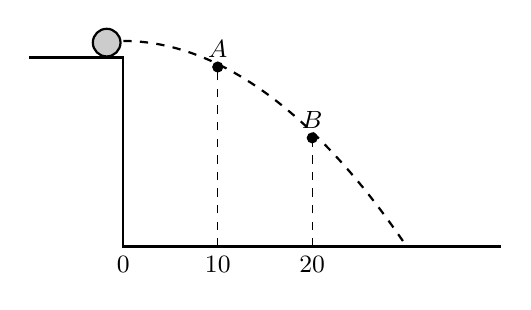
\begin{tikzpicture}[font=\small,scale=1.2]
        %% Surface
        \draw[thick] (-1,0) -- (0,0) -- (0,-2) -- (4,-2);
        %% Labels: 0 m
        \node[anchor=north] at (0,-2) {\SI{0}{\meter}};
        \draw[fill] (1,-0.1) circle (1.5pt) node[anchor=south] {$A$};
        %% Labels: A at 10 m
        \draw[dashed] (1,-2) -- (1,-0.1);
        \node[anchor=north] at (1,-2) {\SI{10}{\meter}};
        %% Labels: B at 20 m
        \draw[fill] (2,-0.85) circle (1.5pt) node[anchor=south] {$B$};
        \draw[dashed] (2,-2) -- (2,-0.85);
        \node[anchor=north] at (2,-2) {\SI{20}{\meter}};
        %% Path
        \node[thick,draw,fill=white!80!black,anchor=south,circle,minimum size=1em] (Car) at (-0.5em,0) {};
        %\draw[->] (Car.east) -- ++ (0:0.75cm) node[pos=0.5,anchor=south] {$v$};
        \draw[thick,dashed] (0,0.5em) parabola bend (0,0.5em) (3,-2);
    \end{tikzpicture}
    \end{center}
    Compared to the horizontal component of the car's velocity at point $A$,
        the horizontal component of the car's velocity at point $B$ is:
    \begin{multicols}{3}
    \begin{choices}
        \wrongchoice{smaller}
        \wrongchoice{greater}
      \correctchoice{the same}
    \end{choices}
    \end{multicols}
\end{question}
}


%% Section June2008
%%--------------------
\element{nysed}{
\begin{question}{June2008-Q02}
    A projectile launched at an angle of \ang{45} above the horizontal travels through the air.
    Compared to the projectile's theoretical path with no air friction,
        the actual trajectory of the projectile with air friction is:
    \begin{choices}
      \correctchoice{lower and shorter}
        \wrongchoice{lower and longer}
        \wrongchoice{higher and shorter}
        \wrongchoice{higher and longer}
    \end{choices}
\end{question}
}

\element{nysed}{
\begin{question}{June2008-Q06}
    Two stones, $A$ and $B$, are thrown horizontally from the top of a cliff.
    Stone $A$ has an initial speed of \SI{15}{\meter\per\second} and stone $B$ has an initial speed of \SI{30}{\meter\per\second}.
    Compared to the time it takes stone $A$ to reach the ground,
        the time it takes stone $B$ to reach the ground is:
    \begin{choices}
      \correctchoice{the same}
        \wrongchoice{twice as great}
        \wrongchoice{half as great}
        \wrongchoice{four times as great}
    \end{choices}
\end{question}
}


%% Section Jan2008
%%--------------------
\element{nysed}{
\begin{question}{Jan2008-Q07}
    Two spheres, $A$ and $B$, are simultaneously projected horizontally from the top of a tower.
    Sphere $A$ has a horizontal speed of \SI{40}{\meter\per\second} and sphere $B$ has a horizontal speed of \SI{20}{\meter\per\second}.
    Which statement best describes the time required for the spheres to reach the ground and the horizontal distance they travel?
    [Neglect friction and assume the ground is level.]
    \begin{choices}
        \wrongchoice{Both spheres hit the ground at the same time and at the same distance from the base of the tower}
      \correctchoice{Both spheres hit the ground at the same time, but sphere $A$ lands twice as far as sphere $B$ from the base of the tower.}
        \wrongchoice{Both spheres hit the ground at the same time, but sphere $B$ lands twice as far as sphere $A$ from the base of the tower.}
        \wrongchoice{Sphere $A$ hits the ground before sphere $B$, and sphere $A$ lands twice as far as sphere $B$ from the base of the tower.}
    \end{choices}
\end{question}
}


%% Section June2007
%%--------------------


%% Section Jan2007
%%--------------------
\element{nysed}{
\begin{question}{Jan2007-Q05}
    A machine launches a tennis ball at an angle of \ang{25} above the horizontal at a speed of \SI{14}{\meter\per\second}.
    The ball returns to level ground.
    Which combination of changes \emph{must} produce an increase in time of flight of a second launch?
    \begin{choices}
      \correctchoice{increase the launch angle and increase the ball's initial speed}
        \wrongchoice{increase the launch angle and decrease the ball's initial speed}
        \wrongchoice{decrease the launch angle and increase the ball's initial speed}
        \wrongchoice{decrease the launch angle and decrease the ball's initial speed}
    \end{choices}
\end{question}
}

\element{nysed}{
\begin{question}{Jan2007-Q07}
    A plane flying horizontally above Earth's surface at \SI{100}{\meter\per\second} drops a crate.
    The crate strikes the ground \SI{30.0}{\second} later.
    What is the magnitude of the horizontal component of the crate's velocity just before it strikes the ground?
    [Neglect friction.]
    \begin{multicols}{2}
    \begin{choices}
      \correctchoice{\SI{100}{\meter\per\second}}
        \wrongchoice{\SI{0}{\meter\per\second}}
        \wrongchoice{\SI{294}{\meter\per\second}}
        \wrongchoice{\SI{394}{\meter\per\second}}
    \end{choices}
    \end{multicols}
\end{question}
}


%% Section June2006
%%--------------------
\element{nysed}{
\begin{question}{June2006-Q44}
    A volleyball hit into the air has an initial speed of \SI{10.}{\meter\per\second}.
    Which vector best represents the angle above the horizontal that the ball should be hit to remain in the air for the greatest amount of time?
    \begin{multicols}{2}
    \begin{choices}
        \AMCboxDimensions{down=-1.5em}
        \correctchoice{
            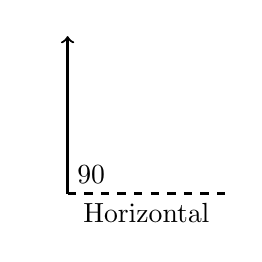
\begin{tikzpicture}
                \draw[white] (-0.5,-0.5) rectangle (2.1,2.1);
                \draw[thick,->] (0,0) -- (90:2cm);
                \draw[thick,dashed] (0,0) -- (0:2cm);
                \node[anchor=north] at (0:1cm) {Horizontal};
                \node[anchor=south west] at (0:0) {\ang{90}};
            \end{tikzpicture}
        }
        \wrongchoice{
            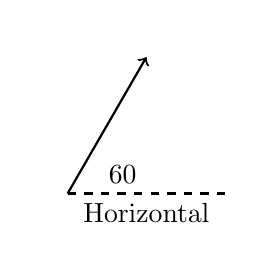
\begin{tikzpicture}
                \draw[white] (-0.5,-0.5) rectangle (2.1,2.1);
                \draw[thick,->] (0,0) -- (60:2cm);
                \draw[thick,dashed] (0,0) -- (0:2cm);
                \node[anchor=north] at (0:1cm) {Horizontal};
                \node[anchor=south east] at (0:1cm) {\ang{60}};
            \end{tikzpicture}
        }
        \wrongchoice{
            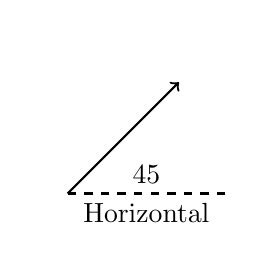
\begin{tikzpicture}
                \draw[white] (-0.5,-0.5) rectangle (2.1,2.1);
                \draw[thick,->] (0,0) -- (45:2cm);
                \draw[thick,dashed] (0,0) -- (0:2cm);
                \node[anchor=north] at (0:1cm) {Horizontal};
                \node[anchor=south] at (0:1cm) {\ang{45}};
            \end{tikzpicture}
        }
        \wrongchoice{
            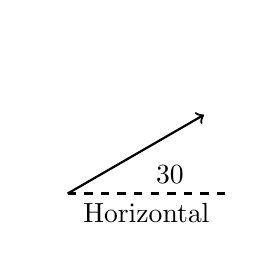
\begin{tikzpicture}
                \draw[white] (-0.5,-0.5) rectangle (2.1,2.1);
                \draw[thick,->] (0,0) -- (30:2cm);
                \draw[thick,dashed] (0,0) -- (0:2cm);
                \node[anchor=north] at (0:1cm) {Horizontal};
                \node[anchor=south west] at (0:1cm) {\ang{30}};
            \end{tikzpicture}
        }
    \end{choices}
    \end{multicols}
\end{question}
}


%% Section Jan2006
%%--------------------


%% Section June2005
%%--------------------
\element{nysed}{
\begin{question}{June2005-Q05}
    A golf ball is hit at an angle of \ang{45} above the horizontal.
    What is the acceleration of the gold ball at the highest point in its trajectory?
    [Neglect friction.]
    \begin{choices}
      \correctchoice{\SI{9.8}{\meter\per\second\squared} downward}
        \wrongchoice{\SI{9.8}{\meter\per\second\squared} upward}
        \wrongchoice{\SI{6.9}{\meter\per\second\squared} horizontal}
        \wrongchoice{\SI{0.0}{\meter\per\second\squared}}
    \end{choices}
\end{question}
}

\element{nysed}{
\begin{question}{June2005-Q07}
    A ball is thrown horizontally at a speed of \SI{24}{\meter\per\second} from the top of a cliff.
    If the ball hits the ground \SI{4.0}{\second} later,
        approximately how high is the cliff?
    \begin{multicols}{2}
    \begin{choices}
      \correctchoice{\SI{78}{\meter}}
        \wrongchoice{\SI{96}{\meter}}
        \wrongchoice{\SI{6.0}{\meter}}
        \wrongchoice{\SI{39}{\meter}}
    \end{choices}
    \end{multicols}
\end{question}
}


%% Section Jan2005
%%--------------------


%% Section June2004
%%--------------------
\element{nysed}{
\begin{question}{June2004-Q04}
    The diagram below represents the path of an object after it was thrown.
    \begin{center}
    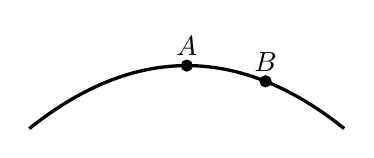
\begin{tikzpicture}
        \draw [very thick,domain=-2:2, samples=50] plot (\x, {2 - 0.20*\x*\x});
        \node [anchor=south] at (0,2) {$A$};
        \draw[fill] (0,2) circle (2pt);
        \node [anchor=south] at (1,1.80) {$B$};
        \draw[fill] (1,1.80) circle (2pt);
    \end{tikzpicture}
    \end{center}
    What happens to the object's acceleration as it travels from $A$ to $B$?
    [Neglect friction.]
    \begin{choices}
      \correctchoice{It remains the same}
        \wrongchoice{It increases}
        \wrongchoice{It decreases}
    \end{choices}
\end{question}
}

\element{nysed}{
\begin{question}{June2004-Q05}
    A \SI{0.2}{\kilo\gram} red ball is thrown horizontally at a speed of \SI{4}{\meter\per\second} from a height of \SI{3}{\meter}.
    A \SI{0.4}{\kilo\gram} green ball is thrown horizontally from the same height at a speed of \SI{8}{\meter\per\second}.
    Compared to the time it takes the red ball to reach the ground,
        the time it takes the green ball to reach the ground is:
    \begin{choices}
      \correctchoice{the same}
        \wrongchoice{one-half as great}
        \wrongchoice{twice as great}
        \wrongchoice{four times as great}
    \end{choices}
\end{question}
}


%% Section Jan2004
%%--------------------
\element{nysed}{
\begin{question}{Jan2004-Q06}
    A child kicks a ball with an initial velocity of \SI{8.5}{\meter\per\second} at an angle of \ang{35} with the horizontal,
        as shown.
    The ball has an initial velocity of \SI{4.9}{\meter\per\second} and a total time of flight of \SI{1.0}{\second}.
    [Neglect air resistance.]
    \begin{center}
        %% Part I of two part question
        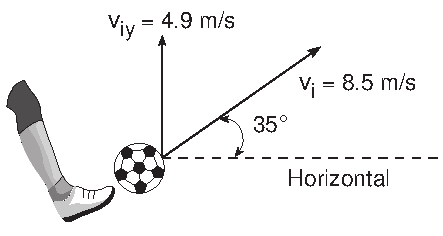
\includegraphics[keepaspectratio,width=0.80\linewidth]{Jan2004-Q06}
    \end{center}
    The horizontal component of the ball's initial velocity is approximately
    \begin{multicols}{2}
    \begin{choices}
      \correctchoice{\SI{7.0}{\meter\per\second}}
        \wrongchoice{\SI{13}{\meter\per\second}}
        \wrongchoice{\SI{3.6}{\meter\per\second}}
        \wrongchoice{\SI{4.9}{\meter\per\second}}
    \end{choices}
    \end{multicols}
\end{question}
}

\element{nysed}{
\begin{question}{Jan2004-Q07}
    A child kicks a ball with an initial velocity of \SI{8.5}{\meter\per\second} at an angle of \ang{35} with the horizontal,
        as shown.
    The ball has an initial velocity of \SI{4.9}{\meter\per\second} and a total time of flight of \SI{1.0}{\second}.
    [Neglect air resistance.]
    \begin{center}
        %% Part II of two part question
        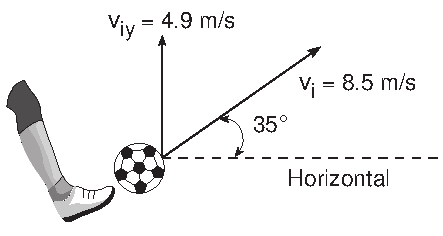
\includegraphics[keepaspectratio,width=0.80\linewidth]{Jan2004-Q06}
    \end{center}
    The maximum height reached by the ball is approximately:
    \begin{multicols}{2}
    \begin{choices}
      \correctchoice{\SI{1.2}{\meter}}
        \wrongchoice{\SI{2.5}{\meter}}
        \wrongchoice{\SI{4.9}{\meter}}
        \wrongchoice{\SI{8.5}{\meter}}
    \end{choices}
    \end{multicols}
\end{question}
}


%% Section June2003
%%--------------------
\element{nysed}{
\begin{question}{June2003-Q04}
    A ball is thrown at an angle of \ang{33} to the horizontal.
    What happens to the magnitude of the ball's vertical acceleration during the total time interval that the ball is in the air?
    \begin{choices}
        \wrongchoice{It decreases, then increases}
        \wrongchoice{It decreases, then remains the same}
        \wrongchoice{It increases, then decreases}
      \correctchoice{It remains the same}
    \end{choices}
\end{question}
}

\element{nysed}{
\begin{question}{June2003-Q06}
    Projectile A is launched horizontally at a speed of \SI{20}{\meter\per\second} from the top of a cliff and strikes a level surface below,
        \SI{3.0}{\second} later.
    Projectile B is launched horizontally from the same location at a speed of \SI{30}{\meter\per\second}.
    The time it takes projectile B to reach the level surface is:
    \begin{multicols}{2}
    \begin{choices}
      \correctchoice{\SI{3.0}{\second}}
        \wrongchoice{\SI{4.5}{\second}}
        \wrongchoice{\SI{2.0}{\second}}
        \wrongchoice{\SI{10}{\second}}
    \end{choices}
    \end{multicols}
\end{question}
}

\element{nysed}{
\begin{question}{June2003-Q07}
    Projectile A is launched horizontally at a speed of \SI{20}{\meter\per\second} from the top of a cliff and strikes a level surface below,
        \SI{3.0}{\second} later.
    Projectile B is launched horizontally from the same location at a speed of \SI{30}{\meter\per\second}.
    Approximately how high is the cliff?
    \begin{multicols}{2}
    \begin{choices}
      \correctchoice{\SI{44}{\meter}}
        \wrongchoice{\SI{29}{\meter}}
        \wrongchoice{\SI{60}{\meter}}
        \wrongchoice{\SI{104}{\meter}}
    \end{choices}
    \end{multicols}
\end{question}
}


%% Section Jan2003
%%--------------------


%% Section Aug2002
%%--------------------
\element{nysed}{
\begin{question}{Aug2002-Q38}
    An archer uses a bow to fire two similar arrows with the same string force.
    One arrow is fired at an angle of \ang{60} with the horizontal,
        and the other is fired at an angle of \ang{45} with the horizontal.
    Compared to the arrow fired at \ang{60},
        the arrow fired at \ang{45} has a:
    \begin{choices}
        \wrongchoice{longer flight time and longer horizontal range}
        \wrongchoice{longer flight time and shorter horizontal range}
      \correctchoice{shorter flight time and longer horizontal range}
        \wrongchoice{shorter flight time and shorter horizontal range}
    \end{choices}
\end{question}
}



%% Section June2002
%%--------------------
\element{nysed}{
\begin{question}{June2002-Q05}
    The diagram below shows a student throwing a baseball horizontally at \SI{25}{\meter\per\second} from a cliff \SI{45}{\meter} above the level ground.
    \begin{center}
    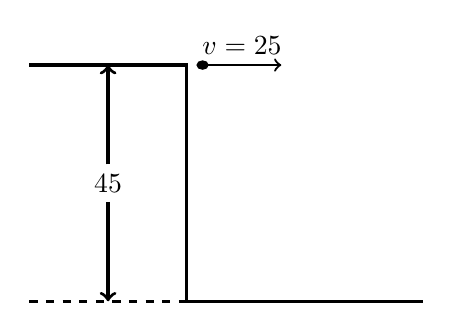
\begin{tikzpicture}[yscale=0.75]
        \draw[very thick] (-2,0) -- (0,0) -- (0,-4) -- (3,-4);
        \draw[fill] (0.2,0.0) circle [radius=2pt];
        \draw[thick,->] (0.2,0.0) -- ++ (0:1)
            node[anchor=south] at ++ (0:-0.5) {$v=\SI{25}{\meter\per\second}$};
        \draw[very thick,dashed] (-2,-4) -- (0,-4);
        \node (A) at (-1,-2.0) {\SI{45}{\meter}};
        \draw[very thick,->] (A) -- (-1,0);
        \draw[very thick,->] (A) -- (-1,-4);
    \end{tikzpicture}
    \end{center}
    Approximately how far from the base of the cliff does the ball hit the ground?
    [Neglect air resistance]
    \begin{multicols}{2}
    \begin{choices}
        \wrongchoice{\SI{45}{\meter}}
      \correctchoice{\SI{75}{\meter}}
        \wrongchoice{\SI{140}{\meter}}
        \wrongchoice{\SI{230}{\meter}}
    \end{choices}
    \end{multicols}
\end{question}
}

\element{nysed}{
\begin{question}{June2002-Q06}
    A projectile is fired from a gun near the surface of Earth.
    The initial velocity of the projectile has a vertical component of \SI{98}{\meter\per\second} and a horizontal component of \SI{49}{\meter\per\second}.
    How long will it take the projectile to reach the highest point in its path?
    \begin{multicols}{2}
    \begin{choices}
        \wrongchoice{\SI{5.0}{\second}}
        \wrongchoice{\SI{10}{\second}}
        \wrongchoice{\SI{20}{\second}}
      \correctchoice{\SI{100}{\second}}
    \end{choices}
    \end{multicols}
\end{question}
}


%% Section Jan2002
%%--------------------
\element{nysed}{
\begin{question}{Jan2002-Q06}
    Which two terms represent a vector quantity and the scalar quantity of the vector's magnitude respectively?
    \begin{choices}
        \wrongchoice{acceleration and velocity}
        \wrongchoice{weight and force}
        \wrongchoice{speed and time}
      \correctchoice{displacement and distance}
    \end{choices}
\end{question}
}

\element{nysed}{
\begin{question}{Jan2002-Q07}
    A \SI{4.0}{\kilo\gram} rock and a \SI{1.0}{\kilo\gram} stone fall freely from rest from a height of \SI{100}{\meter}.
    After they fall for \SI{2.0}{\second},
        the ratio of the rock's speed to the stone's speed is:
    \begin{multicols}{2}
    \begin{choices}
      \correctchoice{$1:1$}
        \wrongchoice{$1:2$}
        \wrongchoice{$2:1$}
        \wrongchoice{$4:1$}
    \end{choices}
    \end{multicols}
\end{question}
}

\newcommand{\nysedJanTwentyZeroTwoQfiftySix}{
\begin{tikzpicture}
    %% Ground
    \draw (-3,0) -- (3,0);
    \node[minimum width=6cm,anchor=north,pattern=north east lines] at (0,0) {};
    \node[anchor=south east] at (3,0) {Ground};
    %\node[anchor=north east] at (3,-1em) {Ground};
    %% Tower
    \draw[thick] (-1.5,0) -- (-0.5,5) -- (0.5,5) -- (1.5,0);
    \draw[thick] (-0.5,5) rectangle (0.5,5.50);
    %% bottom girders
    \draw (-1.5,0) -- ({+1.5-(1.66/5)},1.66);
    \draw (+1.5,0) -- ({-1.5+(1.66/5)},1.66);
    \draw ({-1.5+(1.66/5)},1.66) -- ({1.5-(1.66/5)},1.66);
    %% middle girders
    \draw ({-1.5+(1.66/5)},1.66) -- ({+1.5-(3.33/5)},3.33);
    \draw ({+1.5-(1.66/5)},1.66) -- ({-1.5+(3.33/5)},3.33);
    \draw ({-1.5+(1.66/5)},1.66) -- ({1.5-(1.66/5)},1.66);
    %% top girders
    \draw ({-1.5+(3.33/5)},3.33) -- (+0.5,5);
    \draw ({+1.5-(3.33/5)},3.33) -- (-0.5,5);
    \draw ({-1.5+(3.33/5)},3.33) -- ({1.5-(3.33/5)},3.33);
    %% Ball
    \node[circle,minimum size=1ex,fill,anchor=west] (A) at (0.5,5.25) {};
    \draw[thick,->] (A.east) -- ++(0:1) node[anchor=south,pos=0.5] {\SI{20}{\meter\per\second}};
    %% height
    \draw[dashed] (-0.5,5.25) -- (-3,5.25);
    \draw[latex-latex,shorten <=1pt,shorten >=1pt] (-2.33,0) -- (-2.33,5.25) node[pos=0.5,anchor=center,fill=white] {\SI{60}{\meter}};
\end{tikzpicture}
}

\element{nysed}{
\begin{question}{Jan2002-Q56}
    A ball is thrown horizontally with an initial velocity of \SI{20.0}{\meter\per\second} from the top of a tower \SI{60.0}{\meter} high.
    \begin{center}
        \nysedJanTwentyZeroTwoQfiftySix
    \end{center}
    What is the initial vertical velocity of the ball?
    \begin{multicols}{2}
    \begin{choices}
      \correctchoice{\SI{0}{\meter\per\second}}
        \wrongchoice{\SI{9.81}{\meter\per\second}}
        \wrongchoice{\SI{20.0}{\meter\per\second}}
        \wrongchoice{\SI{60.0}{\meter\per\second}}
    \end{choices}
    \end{multicols}
\end{question}
}

\element{nysed}{
\begin{question}{Jan2002-Q57}
    A ball is thrown horizontally with an initial velocity of \SI{20.0}{\meter\per\second} from the top of a tower \SI{60.0}{\meter} high.
    \begin{center}
        \nysedJanTwentyZeroTwoQfiftySix
    \end{center}
    What is the approximate total time required for the ball to reach the ground?
    [Neglect air resistance]
    \begin{multicols}{2}
    \begin{choices}
        \wrongchoice{\SI{12.2}{\second}}
        \wrongchoice{\SI{2.04}{\second}}
        \wrongchoice{\SI{3.00}{\second}}
      \correctchoice{\SI{3.50}{\second}}
    \end{choices}
    \end{multicols}
\end{question}
}

\element{nysed}{
\begin{question}{Jan2002-Q58}
    A ball is thrown horizontally with an initial velocity of \SI{20.0}{\meter\per\second} from the top of a tower \SI{60.0}{\meter} high.
    \begin{center}
        \nysedJanTwentyZeroTwoQfiftySix
    \end{center}
    What is the horizontal velocity of the ball just before it reaches the ground?
    [Neglect air resistance.]
    \begin{multicols}{2}
    \begin{choices}
        \wrongchoice{\SI{9.81}{\meter\per\second}}
      \correctchoice{\SI{20.0}{\meter\per\second}}
        \wrongchoice{\SI{34.3}{\meter\per\second}}
        \wrongchoice{\SI{68.6}{\meter\per\second}}
    \end{choices}
    \end{multicols}
\end{question}
}

\newcommand{\nysedJanTwentyZeroTwoQSixtyTwo}{
%% NOTE: TODO: draw tikz
\begin{tikzpicture}
    %% ground
    \draw (-3,0) -- (3,0);
    \node[minimum width=6cm,anchor=north,pattern=north east lines] at (0,0) {};
    %% Body
    %% ball
\end{tikzpicture}
}

\element{nysed}{
\begin{question}{Jan2002-Q62}
    A golf ball leaves a golf club with an initial velocity of \SI{40}{\meter\per\second} at an angle of \ang{40} with respect to the horizontal.
    \begin{center}
        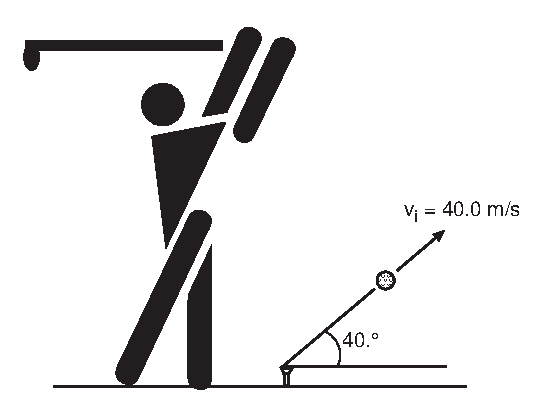
\includegraphics[keepaspectratio,scale=0.90]{Jan2002-Q62}
    \end{center}
    What is the vertical component of the golf ball's initial velocity?
    \begin{multicols}{2}
    \begin{choices}
      \correctchoice{\SI{25.7}{\meter\per\second}}
        \wrongchoice{\SI{30.6}{\meter\per\second}}
        \wrongchoice{\SI{40.0}{\meter\per\second}}
        \wrongchoice{\SI{61.3}{\meter\per\second}}
    \end{choices}
    \end{multicols}
\end{question}
}

\element{nysed}{
\begin{question}{Jan2002-Q63}
    A golf ball leaves a golf club with an initial velocity of \SI{40}{\meter\per\second} at an angle of \ang{40} with respect to the horizontal.
    \begin{center}
        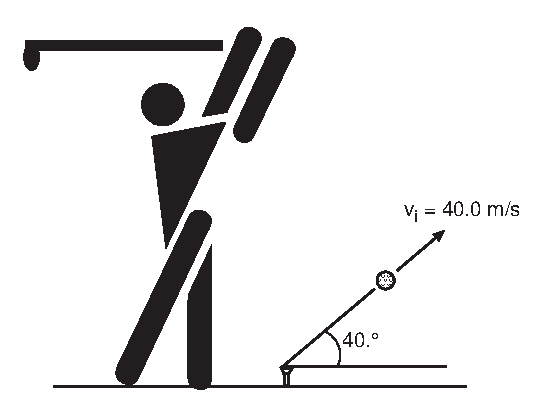
\includegraphics[keepaspectratio,scale=0.90]{Jan2002-Q62}
    \end{center}
    What is the total horizontal distance traveled by the golf ball during the first \SI{2.5}{\second} of its flight?
    \begin{multicols}{2}
    \begin{choices}
        \wrongchoice{\SI{100}{\meter}}
      \correctchoice{\SI{76.6}{\meter}}
        \wrongchoice{\SI{64.3}{\meter}}
        \wrongchoice{\SI{40.0}{\meter}}
    \end{choices}
    \end{multicols}
\end{question}
}


%% Section June2001
%%--------------------
\element{nysed}{
\begin{question}{June2001-Q58}
    A red ball and a green ball are simultaneously thrown horizontally from the same height.
    The red ball has an initial speed of \SI{40}{\meter\per\second} and the green ball has an initial speed of \SI{20}{\meter\per\second}.
    Compared to the time it takes the red ball to reach the ground,
        the time it takes the green ball to reach the ground will be:
    \begin{choices}
      \correctchoice{the same}
        \wrongchoice{half as much}
        \wrongchoice{twice as much}
        \wrongchoice{four times as much}
    \end{choices}
\end{question}
}

\element{nysed}{
\begin{question}{June2001-Q59}
    A baseball player throws a ball horizontally.
    Which statement best describes the ball's motion after it is thrown?
    [Neglect the effect of friction.]
    \begin{choices}
        \wrongchoice{Its vertical speed remains the same, and its horizontal speed increases.}
        \wrongchoice{Its vertical speed remains the same, and its horizontal speed remains the same.}
        \wrongchoice{Its vertical speed increases, and its horizontal speed increases.}
      \correctchoice{Its vertical speed increases, and its horizontal speed remains the same.}
    \end{choices}
\end{question}
}


%% Section Jan2001
%%--------------------
\element{nysed}{
\begin{question}{Jan2001-Q58}
    A red ball and a green ball are simultaneously thrown horizontally from the same height.
    the red ball has an initial speed of \SI{40}{\meter\per\second} and the green ball has an initial speed of \SI{20}{\meter\per\second}.
    Compared to the the time it takes the red ball to reach the ground,
        the time it takes the green ball to reach the ground will be:
    \begin{choices}
      \correctchoice{the same}
        \wrongchoice{twice as much}
        \wrongchoice{half as much}
        \wrongchoice{four times as much}
    \end{choices}
\end{question}
}

\element{nysed}{
\begin{question}{Jan2001-Q62}
    The path of a projectile fired at a \ang{30} to the horizontal is best described as:
    \begin{multicols}{2}
    \begin{choices}
      \correctchoice{parabolic}
        \wrongchoice{linear}
        \wrongchoice{circular}
        \wrongchoice{hyperbolic}
    \end{choices}
    \end{multicols}
\end{question}
}


%% Section June2000
%%--------------------
\newcommand{\nysedJuneTwentyZeroZeroQFiftySix}{
%% NOTE: TODO: draw tikz
\begin{tikzpicture}
    %% Cannon
    %% trajectory
\end{tikzpicture}
}

\element{nysed}{
\begin{question}{June2000-Q56}
    A machine launches a tennis ball at an angle of \ang{45} with the horizontal,
        as shown.
    The ball has an initial vertical velocity of \SI{9.0}{\meter\per\second} and an initial horizontal velocity of \SI{9.0}{\meter\per\second}.
    The ball reaches its maximum height \SI{0.92}{\second} after its launch.
    [Neglect air resistance and assume the ball lands at the same height above the ground from which it was launched.]
    \begin{center}
        %\nysedJuneTwentyZeroZeroQFiftySix}{
        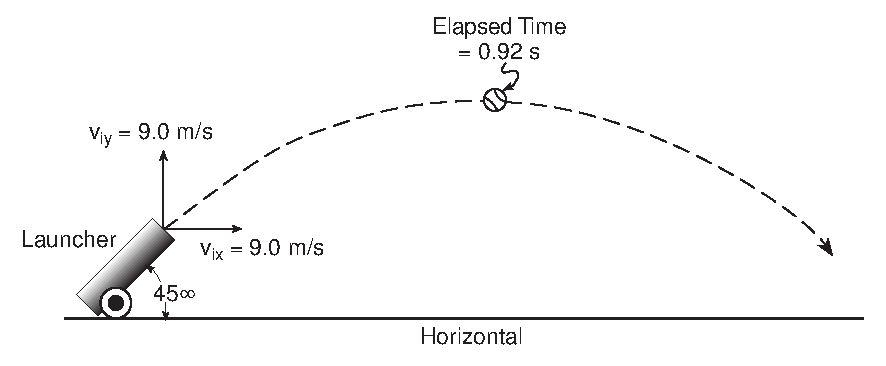
\includegraphics[keepaspectratio,width=\columnwidth]{June2000-Q56}
    \end{center}
    The speed of the tennis ball as it leaves the launcher is approximately:
    \begin{multicols}{2}
    \begin{choices}
        \wrongchoice{\SI{4.5}{\meter\per\second}}
      \correctchoice{\SI{13}{\meter\per\second}}
        \wrongchoice{\SI{8.3}{\meter\per\second}}
        \wrongchoice{\SI{18}{\meter\per\second}}
    \end{choices}
    \end{multicols}
\end{question}
}

\element{nysed}{
\begin{question}{June2000-Q57}
    A machine launches a tennis ball at an angle of \ang{45} with the horizontal,
        as shown.
    The ball has an initial vertical velocity of \SI{9.0}{\meter\per\second} and an initial horizontal velocity of \SI{9.0}{\meter\per\second}.
    The ball reaches its maximum height \SI{0.92}{\second} after its launch.
    [Neglect air resistance and assume the ball lands at the same height above the ground from which it was launched.]
    \begin{center}
        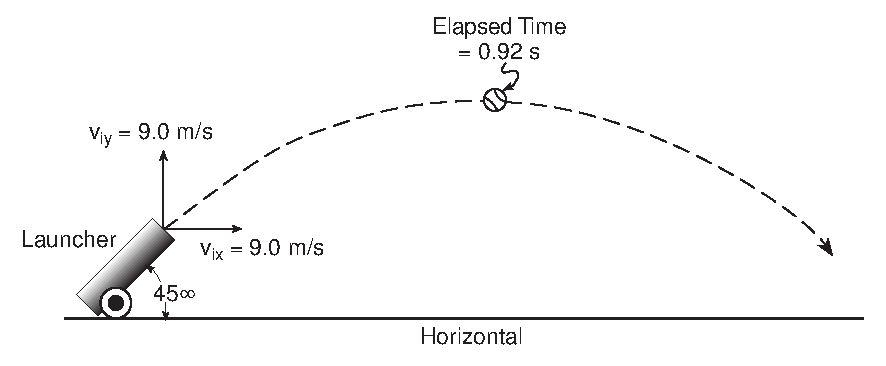
\includegraphics[keepaspectratio,width=\columnwidth]{June2000-Q56}
    \end{center}
    The total horizontal distance traveled by the tennis ball during the entire time it is in the air is approximately:
    \begin{multicols}{2}
    \begin{choices}
        \wrongchoice{\SI{23}{\meter}}
        \wrongchoice{\SI{17}{\meter}}
      \correctchoice{\SI{8.3}{\meter}}
        \wrongchoice{\SI{4.1}{\meter}}
    \end{choices}
    \end{multicols}
\end{question}
}

\element{nysed}{
\begin{question}{June2000-Q58}
    A machine launches a tennis ball at an angle of \ang{45} with the horizontal,
        as shown.
    The ball has an initial vertical velocity of \SI{9.0}{\meter\per\second} and an initial horizontal velocity of \SI{9.0}{\meter\per\second}.
    The ball reaches its maximum height \SI{0.92}{\second} after its launch.
    [Neglect air resistance and assume the ball lands at the same height above the ground from which it was launched.]
    \begin{center}
        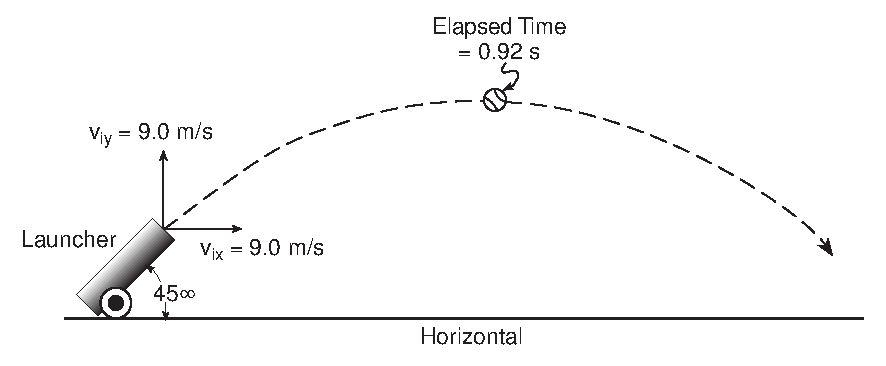
\includegraphics[keepaspectratio,width=\columnwidth]{June2000-Q56}
    \end{center}
    The speed at which the launcher fires tennis balls is constant,
        but the angle between the launcher and the horizontal can be varied.
    As the angle is decreased from \ang{45} to \ang{30},
        the range of the tennis balls:
    \begin{choices}
      \correctchoice{decreases}
        \wrongchoice{increases}
        \wrongchoice{remains the same}
    \end{choices}
\end{question}
}

\element{nysed}{
\begin{question}{June2000-Q59}
    A \SI{2}{\kilo\gram} block is dropped from the roof of a tall building at the same time a \SI{6}{\kilo\gram} ball is thrown horizontally from the same height.
    Which statement best describes the motion of the block and the motion of the ball? [Neglect air resistance]
    \begin{choices}
        \wrongchoice{The \SI{2}{\kilo\gram} block hits the ground first because it has no horizontal velocity.}
        \wrongchoice{The \SI{6}{\kilo\gram} block hits the ground first because it has more mass.}
        \wrongchoice{The \SI{6}{\kilo\gram} block hits the ground first because it is round.}
      \correctchoice{The block and the ball hit the ground at the same time because they have the same vertical acceleration}
    \end{choices}
\end{question}
}


%% Section June1999
%%--------------------
\element{nysed}{
\begin{question}{June1999-Q58}
    The diagram below shows the muzzle of a cannon located \SI{50}{\meter} above the ground.
    When the cannon is fired, a ball leaves the muzzle with an initial speed of \SI{250}{\meter\per\second}.
    [Neglect air resistance]
    \begin{center}
    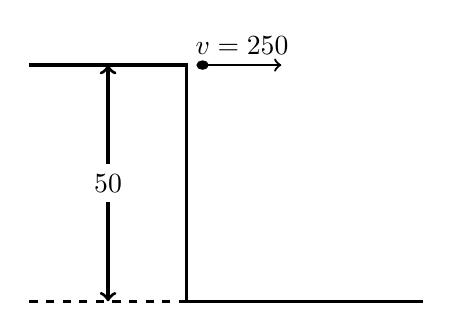
\begin{tikzpicture}[yscale=0.75]
        \draw[very thick] (-2,0) -- (0,0) -- (0,-4) -- (3,-4);
        \draw[fill] (0.2,0.0) circle [radius=2pt];
        \draw[thick,->] (0.2,0.0) -- ++ (0:1)
            node[anchor=south] at ++ (0:-0.5) {$v=\SI{250}{\meter\per\second}$};
        \draw[very thick,dashed] (-2,-4) -- (0,-4);
        \node (A) at (-1,-2.0) {\SI{50}{\meter}};
        \draw[very thick,->] (A) -- (-1,0);
        \draw[very thick,->] (A) -- (-1,-4);
    \end{tikzpicture}
    \end{center}
    Which action would most likely increase the time of flight of the ball fired by the cannon?
    \begin{choices}
        \wrongchoice{pointing the muzzle of the cannon toward the ground}
        \wrongchoice{moving the cannon closer to the edge of the cliff}
      \correctchoice{positioning the cannon higher above the ground}
        \wrongchoice{giving the ball a greater initial horizontal velocity}
    \end{choices}
\end{question}
}

\element{nysed}{
\begin{question}{June1999-Q62}
    In the diagram below,
        a stationary observer on the ground watches as a seagull flying horizontally to the right drops a clamshell.
    \begin{center}
        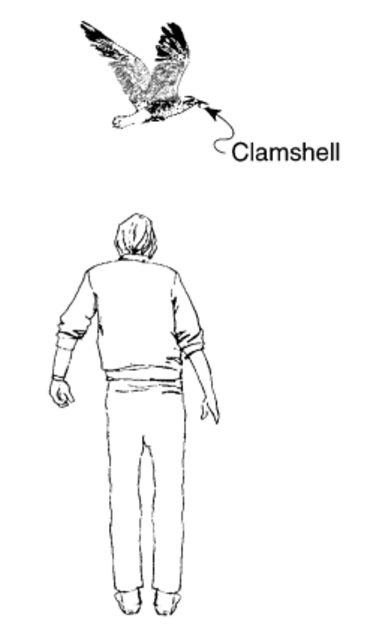
\includegraphics[keepaspectratio,scale=0.66]{June1999-Q62}
    \end{center}
    Which diagram best represents the path of the falling clamshell as seen by the observer?
    [Neglect air resistance]
    \begin{multicols}{2}
    \begin{choices}
        \AMCboxDimensions{down=-0.8cm}
        \wrongchoice{
            \begin{tikzpicture}[scale=2]
                \draw[dashed,white!60!black] (0,0) rectangle (1,1);
                \draw[thick,->] (0.5,1) -- (0.5,0);
            \end{tikzpicture}
        }
        \wrongchoice{
            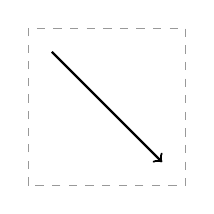
\begin{tikzpicture}[scale=2]
                \draw[dashed,white!60!black] (0,0) rectangle (1,1);
                \draw[thick,->] (0.15,0.85) -- (0.85,0.15);
            \end{tikzpicture}
        }
        \wrongchoice{
            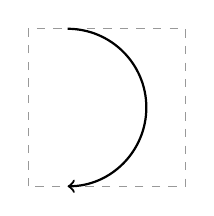
\begin{tikzpicture}[scale=2]
                \draw[dashed,white!60!black] (0,0) rectangle (1,1);
                \draw[thick,->] (0.25,1) arc (90:-90:0.50);
            \end{tikzpicture}
        }
        \correctchoice{
            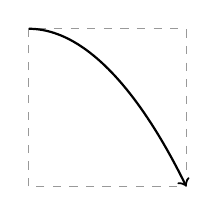
\begin{tikzpicture}[scale=2]
                \draw[dashed,white!60!black] (0,0) rectangle (1,1);
                \draw[thick,->] (0,1) parabola (1,0);
            \end{tikzpicture}
        }
    \end{choices}
    \end{multicols}
\end{question}
}


%% Section June1998
%%--------------------
\newcommand{\nysedJuneNineteenNinetyNineQFiftySix}{
%% NOTE: TODO: draw tikz
\begin{tikzpicture}
\end{tikzpicture}
}

\element{nysed}{
\begin{question}{June1998-Q56}
    A student standing on a knoll throws a snowball horizontally \SI{4.5}{\meter} above the level ground towards a smokestack \SI{15}{\meter} away.
    The snowball hits the smokestack \SI{0.65}{\second} after being released.
    [Neglect air resistance]
    \begin{center}
        %\nysedJuneNineteenNinetyNineQFiftySix
        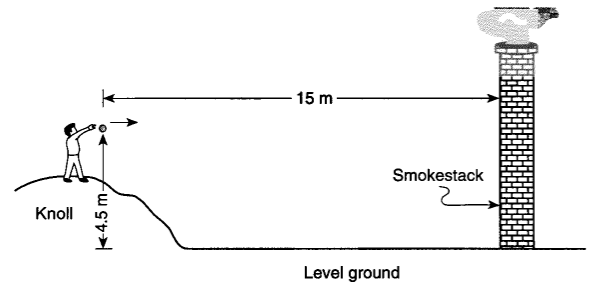
\includegraphics[keepaspectratio,width=\linewidth]{June1998-Q56}
    \end{center}
    Approximately how far above the level ground does the snowball hit the smokestack?
    \begin{multicols}{2}
    \begin{choices}
        \wrongchoice{\SI{0.0}{\meter}}
        \wrongchoice{\SI{0.4}{\meter}}
      \correctchoice{\SI{2.4}{\meter}}
        \wrongchoice{\SI{4.5}{\meter}}
    \end{choices}
    \end{multicols}
\end{question}
}

\element{nysed}{
\begin{question}{June1998-Q57}
    A student standing on a knoll throws a snowball horizontally \SI{4.5}{\meter} above the level ground towards a smokestack \SI{15}{\meter} away.
    The snowball hits the smokestack \SI{0.65}{\second} after being released.
    [Neglect air resistance]
    \begin{center}
        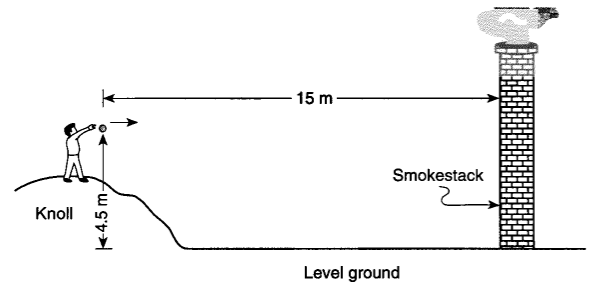
\includegraphics[keepaspectratio,width=0.95\linewidth]{June1998-Q56}
    \end{center}
    At the instant the snowball is released,
        the horizontal component of its velocity is approximately:
    \begin{multicols}{2}
    \begin{choices}
        \wrongchoice{\SI{6.9}{\meter\per\second}}
        \wrongchoice{\SI{9.8}{\meter\per\second}}
        \wrongchoice{\SI{17}{\meter\per\second}}
      \correctchoice{\SI{23}{\meter\per\second}}
    \end{choices}
    \end{multicols}
\end{question}
}

\element{nysed}{
\begin{question}{June1998-Q62}
    The diagram below shows a projectile moving with speed $v$ at the top of its trajectory.
    \begin{center}
    \begin{tikzpicture}
        %% Ground
        \draw[thick] (-3.5,0) -- (3.5,0);
        \node[anchor=north,fill,pattern=north east lines,minimum width=7cm, minimum height=0.05cm] at (0,0) {};
        \node[anchor=north] at (0,-1em) {Ground};
        %% Path: y = 2/9 x^2, y' = 4/9 x, dy/dx (2) = 12/9, atan(12/9) = 53
        \draw[thick,dashed] (-3,0) parabola bend (0,2) (3,0);
        \draw[thick,->] (-3,0) -- ++(53:1);
        %% Projectile
        \draw[fill] (0,2) circle (3pt) node[anchor=north,yshift=-3pt,font=\small] {Projectile};
        \draw[thick,->] (-0.5,2.4) -- (0.5,2.4) node[pos=0.5,anchor=south] {$v$};
    \end{tikzpicture}
    \end{center}
    Which vector best represents the acceleration of the projectile in the position shown?
    \begin{multicols}{4}
    \begin{choices}
        \AMCboxDimensions{down=-0.2cm}
        \correctchoice{
            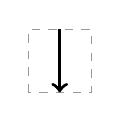
\begin{tikzpicture}[scale=0.4]
                \draw[dashed,white!60!black] (0,0) rectangle (2,2);
                \draw[very thick,->] (1,2) -- (1,0);
            \end{tikzpicture}
        }
        \wrongchoice{
            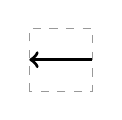
\begin{tikzpicture}[scale=0.4]
                \draw[dashed,white!60!black] (0,0) rectangle (2,2);
                \draw[very thick,->] (2,1) -- (0,1);
            \end{tikzpicture}
        }
        \wrongchoice{
            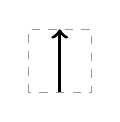
\begin{tikzpicture}[scale=0.4]
                \draw[dashed,white!60!black] (0,0) rectangle (2,2);
                \draw[very thick,->] (1,0) -- (1,2);
            \end{tikzpicture}
        }
        \wrongchoice{
            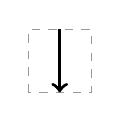
\begin{tikzpicture}[scale=0.4]
                \draw[dashed,white!60!black] (0,0) rectangle (2,2);
                \draw[very thick,->] (1,2) -- (1,0);
            \end{tikzpicture}
        }
    \end{choices}
    \end{multicols}
\end{question}
}


%% Section June1997
%%--------------------
\element{nysed}{
\begin{question}{June1997-Q62}
    Projectiles are fired from different angles with the same speed of \SI{14}{\meter\per\second}.
    The graph below shows the range of the projectiles as a function of the original angle of inclination to the ground, neglecting air resistance.
    \begin{center}
    \begin{tikzpicture}
        \begin{axis}[
            axis y line=left,
            axis x line=bottom,
            axis line style={->},
            xlabel={Angle},
            x unit=\si{\degree},
            xtick={0,10,20,30,40,50,60,70,80,90},
            ylabel={Range},
            y unit=\si{\meter},
            ytick={0,5,10,15,20},
            grid=major,
            xmin=0,xmax=90,
            ymin=0,ymax=21,
            width=0.8\columnwidth,
            height=0.5\columnwidth,
        ]
        \addplot[line width=1pt,domain=0:90]{20*sin(2*x)};
        \end{axis}
    \end{tikzpicture}
    \end{center}
    The graph shows that the range of the projectile is:
    \begin{choices}
        \wrongchoice{the same for all angles.}
        \wrongchoice{the same for angles of \ang{20} and \ang{80}.}
      \correctchoice{greatest for an angle of \ang{45}.}
        \wrongchoice{greatest for an angle of \ang{90}.}
    \end{choices}
\end{question}
}

\element{nysed}{
\begin{question}{June1997-Q64}
    Four different balls are thrown horizontally off the top of four cliffs.
    In which diagram does the ball have the shortest time of flight?
    \begin{multicols}{2}
    \begin{choices}
        \AMCboxDimensions{down=-1cm}
        \correctchoice{
            \begin{tikzpicture}[font=\footnotesize]
                \draw[dashed,white!90!black] (-1.5,-1.2em) rectangle (1.5,4.3);
                %% Cliff
                \draw[thick] (-1,1) -- (0,1) -- (0,0) -- (1,0);
                \node[anchor=south,rotate=270] at (0,0.5) {Cliff};
                \node[anchor=north,rotate=0.0] at (0.5,0) {Ground};
                %% Height
                \draw[<->] (-0.9,1) -- (-0.9,0) node[pos=0.5,anchor=center,fill=white] {\SI{125}{\meter}};
                %% Mass
                \draw[fill] (0,1.33) circle (1.5pt) node[anchor=east] {\SI{1.0}{\kilo\gram}};
                %% velocity
                \draw[thick,->] (0,1.33) -- ++ (0:1) node[pos=0.5,anchor=south] {\SI{50}{\meter\per\second}};
            \end{tikzpicture}
        }
        \wrongchoice{
            \begin{tikzpicture}[font=\footnotesize]
                \draw[dashed,white!90!black] (-1.5,-1.2em) rectangle (1.5,4.3);
                %% Cliff
                \draw[thick] (-1,2) -- (0,2) -- (0,0) -- (1,0);
                \node[anchor=south,rotate=270] at (0,1.0) {Cliff};
                \node[anchor=north,rotate=0.0] at (0.5,0) {Ground};
                %% Height
                \draw[<->] (-0.9,2) -- (-0.9,0) node[pos=0.5,anchor=center,fill=white] {\SI{250}{\meter}};
                %% Mass
                \draw[fill] (0,2.33) circle (1.5pt) node[anchor=east] {\SI{0.5}{\kilo\gram}};
                %% velocity
                \draw[thick,->] (0,2.33) -- ++ (0:1) node[pos=0.5,anchor=south] {\SI{40}{\meter\per\second}};
            \end{tikzpicture}
        }
        \wrongchoice{
            \begin{tikzpicture}[font=\footnotesize]
                \draw[dashed,white!90!black] (-1.5,-1.2em) rectangle (1.5,4.3);
                %% Cliff
                \draw[thick] (-1,3) -- (0,3) -- (0,0) -- (1,0);
                \node[anchor=south,rotate=270] at (0,1.5) {Cliff};
                \node[anchor=north,rotate=0.0] at (0.5,0) {Ground};
                %% Height
                \draw[<->] (-0.9,3) -- (-0.9,0) node[pos=0.5,anchor=center,fill=white] {\SI{375}{\meter}};
                %% Mass
                \draw[fill] (0,3.33) circle (1.5pt) node[anchor=east] {\SI{0.25}{\kilo\gram}};
                %% velocity
                \draw[thick,->] (0,3.33) -- ++ (0:1) node[pos=0.5,anchor=south] {\SI{35}{\meter\per\second}};
            \end{tikzpicture}
        }
        \wrongchoice{
            \begin{tikzpicture}[font=\footnotesize]
                \draw[dashed,white!90!black] (-1.5,-1.2em) rectangle (1.5,4.3);
                %% Cliff
                \draw[thick] (-1,3.6) -- (0,3.6) -- (0,0) -- (1,0);
                \node[anchor=south,rotate=270] at (0,1.5) {Cliff};
                \node[anchor=north,rotate=0.0] at (0.5,0) {Ground};
                %% Height
                \draw[<->] (-0.9,3.6) -- (-0.9,0) node[pos=0.5,anchor=center,fill=white] {\SI{450}{\meter}};
                %% Mass
                \draw[fill] (0,3.9) circle (1.5pt) node[anchor=east] {\SI{0.1}{\kilo\gram}};
                %% velocity
                \draw[thick,->] (0,3.9) -- ++ (0:1) node[pos=0.5,anchor=south] {\SI{35}{\meter\per\second}};
            \end{tikzpicture}
        }
    \end{choices}
    \end{multicols}
\end{question}
}


%% Section June1996
%%--------------------
\newcommand{\JuneNineteenNinetySixQFiftySix}{
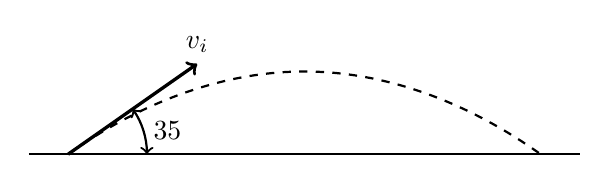
\begin{tikzpicture}
    %% NOTE: useful reference
    %% \frac{h}{R} = \frac{\tan\theta}{4}
    \draw[thick] (-3.5,0) -- (3.5,0);
    \draw[thick,dashed] (-3,0) parabola bend (0,1.05) (3,0);
    \draw[very thick,->] (-3,0) -- ++ (35:2.0cm) node[pos=1.0,anchor=south] {$v_i$};
    \draw[thick,<->] (-2,0) arc (0:35:1cm) node[pos=0.5,anchor=west] {\ang{35}};
\end{tikzpicture}
}

\element{nysed}{
\begin{question}{June1996-Q56}
    A cannon elevated at an angle of \ang{35} to the horizontal fires a cannonball,
        which travels the path shown in the diagram below.
    [Neglect air resistance and assume the ball lands at the same height above the ground from which it was launched.]
    \begin{center}
        \JuneNineteenNinetySixQFiftySix
    \end{center}
    If the ball lands \SI{7.0e2}{\meter} from the cannon \SI{10}{\second} after it was fired,
        what is the horizontal component of its initial velocity?
    \begin{multicols}{2}
    \begin{choices}
      \correctchoice{\SI{70}{\meter\per\second}}
        \wrongchoice{\SI{49}{\meter\per\second}}
        \wrongchoice{\SI{35}{\meter\per\second}}
        \wrongchoice{\SI{7.0}{\meter\per\second}}
    \end{choices}
    \end{multicols}
\end{question}
}

\element{nysed}{
\begin{question}{June1996-Q57}
    A cannon elevated at an angle of \ang{35} to the horizontal fires a cannonball,
        which travels the path shown in the diagram below.
    [Neglect air resistance and assume the ball lands at the same height above the ground from which it was launched.]
    \begin{center}
        \JuneNineteenNinetySixQFiftySix
    \end{center}
    If the ball's time of flight is \SI{10}{\second},
        what is the vertical component of its initial velocity?
    \begin{multicols}{2}
    \begin{choices}
        \wrongchoice{\SI{9.8}{\meter\per\second}}
      \correctchoice{\SI{49}{\meter\per\second}}
        \wrongchoice{\SI{70}{\meter\per\second}}
        \wrongchoice{\SI{98}{\meter\per\second}}
    \end{choices}
    \end{multicols}
\end{question}
}

\element{nysed}{
\begin{question}{June1996-Q58}
    A cannon elevated at an angle of \ang{35} to the horizontal fires a cannonball,
        which travels the path shown in the diagram below.
    [Neglect air resistance and assume the ball lands at the same height above the ground from which it was launched.]
    \begin{center}
        \JuneNineteenNinetySixQFiftySix
    \end{center}
    If the angle of elevation of the cannon is decreased from \ang{35} to \ang{30},
        the vertical component of the ball's initial velocity will:
    \begin{choices}
        \wrongchoice{decrease and its horizontal will decrease.}
      \correctchoice{decrease and its horizontal will increase.}
        \wrongchoice{increase and its horizontal will decrease.}
        \wrongchoice{increase and its horizontal will increase.}
    \end{choices}
\end{question}
}

\element{nysed}{
\begin{question}{June1996-Q65}
    A ball is projected horizontally to the right from a height of \SI{50}{\meter},
        as shown in the diagram below.
    \begin{center}
    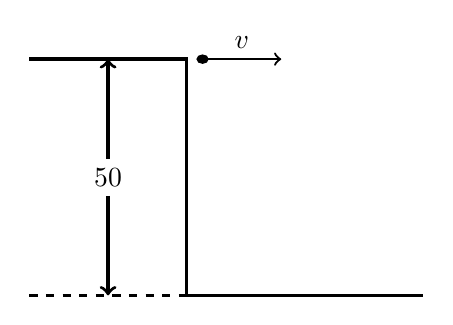
\begin{tikzpicture}[yscale=0.75]
        \draw[very thick] (-2,0) -- (0,0) -- (0,-4) -- (3,-4);
        \draw[fill] (0.2,0.0) circle [radius=2pt];
        \draw[thick,->] (0.2,0.0) -- ++ (0:1)
            node[anchor=south] at ++ (0:-0.5) {$v$};
        \draw[very thick,dashed] (-2,-4) -- (0,-4);
        \node (A) at (-1,-2.0) {\SI{50}{\meter}};
        \draw[very thick,->] (A) -- (-1,0);
        \draw[very thick,->] (A) -- (-1,-4);
    \end{tikzpicture}
    \end{center}
    Which diagram best represents the position of the ball at \SI{1.0}{\second} intervals?
    [Neglect air resistance.]
    \begin{multicols}{2}
    \begin{choices}
        \AMCboxDimensions{down=-1.5em}
        \correctchoice{
            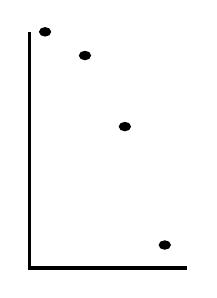
\begin{tikzpicture}[yscale=0.75]
                \draw[very thick] (0,0) -- (0,-4) -- (2,-4);
                \draw[domain=0:3.8,samples=4,mark=*,only marks] plot ({0.2+0.4*\x}, {-0.25*\x*\x});
            \end{tikzpicture}
        }
        \wrongchoice{
            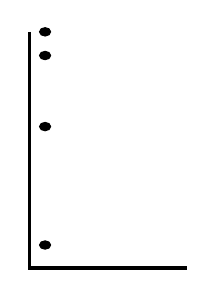
\begin{tikzpicture}[yscale=0.75]
                \draw[very thick] (0,0) -- (0,-4) -- (2,-4);
                \draw[domain=0:3.8,samples=4,mark=*,only marks] plot (0.2, {-0.25*\x*\x});
            \end{tikzpicture}
        }
        \wrongchoice{
            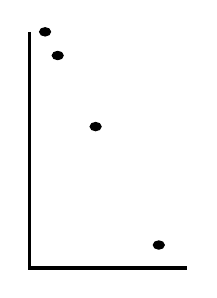
\begin{tikzpicture}[yscale=0.75]
                \draw[very thick] (0,0) -- (0,-4) -- (2,-4);
                \draw[domain=0:3.8,samples=4,mark=*,only marks] plot ({0.2+0.10*\x*\x}, {-0.25*\x*\x});
            \end{tikzpicture}
        }
        \wrongchoice{
            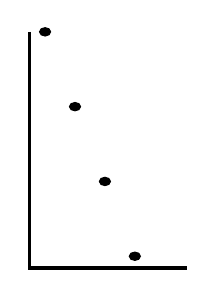
\begin{tikzpicture}[yscale=0.75]
                \draw[very thick] (0,0) -- (0,-4) -- (2,-4);
                \draw[domain=0:3.8,samples=4,mark=*,only marks] plot ({0.2+0.3*\x}, {-1.0*\x});
            \end{tikzpicture}
        }
    \end{choices}
    \end{multicols}
\end{question}
}


%% Section June1995
%%--------------------
\element{nysed}{
\begin{question}{June1995-Q64}
    A cannon with a muzzle velocity of \SI{800}{\meter\per\second} fires a cannonball at an angle of \ang{30} above the horizontal.
    What is the vertical component of the cannonball's velocity at it leaves the cannon?
    \begin{multicols}{2}
    \begin{choices}
        %\wrongchoice{\SI{0.0}{\meter\per\second}}
        \wrongchoice{zero}
      \correctchoice{\SI{250}{\meter\per\second}}
        \wrongchoice{\SI{433}{\meter\per\second}}
        \wrongchoice{\SI{500}{\meter\per\second}}
    \end{choices}
    \end{multicols}
\end{question}
}


%% Section June1994
%%--------------------


%% Section June1989
%%--------------------
\element{nysed}{
\begin{question}{June1989-Q61}
    A \SI{1}{\kilo\gram} object is thrown horizontally and a \SI{2}{\kilo\gram} object is dropped vertically at the same instant and from the same point above the ground.
    If friction is neglected,
        at any given instant both objects will have the same:
    \begin{multicols}{2}
    \begin{choices}
        \wrongchoice{kinetic energy}
        \wrongchoice{momentum}
        \wrongchoice{total velocity}
      \correctchoice{height}
    \end{choices}
    \end{multicols}
\end{question}
}

\element{nysed}{
\begin{question}{June1989-Q69}
    A projectile is launched at an angle of \ang{60} above the horizontal.
    Compared to the vertical component of the initial velocity of the projectile,
        the vertical component of the projectile's velocity when it is has reached its maximum height is:
    \begin{multicols}{3}
    \begin{choices}
      \correctchoice{less}
        \wrongchoice{greater}
        \wrongchoice{the same}
    \end{choices}
    \end{multicols}
\end{question}
}



\endinput


